\section{Experiments}

  In order to support the claim that our algorithm is agnostic to the
  ConvNet architecture as well as hardware it is running on decide to
  benchmark the convolutional layers of state of the art, top
  performing networks used for -- (1) 2D object detection, (2) 2D
  image segmentation and (3) spatiotemporal feature learning (3D)

  \begin{table} \centering
    \setlength\tabcolsep{2.5pt}
    \begin{tabular}{cr !{\vrule width0.8pt} cccccc  }
      &  & B & F & F' & Image Size & Padding & Kernel Size  \\
      \hline
      \multirow{5}{*}{\rotatebox{90}{\textbf{VGG-a}}}
      & C2 & 64  & 64  &  128 & $\angled{112,112}$ & $\angled{1,1}$ & $\angled{3,3}$ \\
      & C3 & 64  & 128 &  256 & $\angled{56,56}$   & $\angled{1,1}$ & $\angled{3,3}$ \\
      & C4 & 64  & 256 &  256 & $\angled{56,56}$   & $\angled{1,1}$ & $\angled{3,3}$ \\
      & C5 & 64  & 256 &  512 & $\angled{28,28}$   & $\angled{1,1}$ & $\angled{3,3}$ \\
      & C6 & 64  & 512 &  512 & $\angled{28,28}$   & $\angled{1,1}$ & $\angled{3,3}$ \\
      \hline
      \multirow{5}{*}{\rotatebox{90}{\textbf{U-Net}}}
      & C1b & 1  & 64  &  64 & $\angled{570,570}$  & $\angled{0,0}$ & $\angled{3,3}$ \\
      & C2b & 1  & 128 &  128 & $\angled{282,282}$ & $\angled{0,0}$ & $\angled{3,3}$ \\
      & C3b & 1  & 256 &  256 & $\angled{138,138}$ & $\angled{0,0}$ & $\angled{3,3}$ \\
      & C4b & 1  & 512 &  512 & $\angled{66,66}$   & $\angled{0,0}$ & $\angled{3,3}$ \\
      & C5b & 1  & 1024 &  1024 & $\angled{30,30}$ & $\angled{0,0}$ & $\angled{3,3}$ \\
      \hline
      \multirow{5}{*}{\rotatebox{90}{\textbf{VGG-a}}}
      & C2a & 32  & 64  &  128 & $\angled{16,56,56}$ & $\angled{1,1,1}$ & $\angled{3,3,3}$ \\
      & C3a & 32  & 128 &  256 & $\angled{8,28,28}$ & $\angled{1,1,1}$ & $\angled{3,3,3}$ \\
      & C3b & 32  & 256 &  256 & $\angled{8,28,28}$ & $\angled{1,1,1}$ & $\angled{3,3,3}$ \\
      & C4a & 32  & 256 &  512 & $\angled{4,14,14}$ & $\angled{1,1,1}$ & $\angled{3,3,3}$ \\
      & C4b & 32  & 512 &  512 & $\angled{4,14,14}$ & $\angled{1,1,1}$ & $\angled{3,3,3}$ \\
      \hline
      \multirow{5}{*}{\rotatebox{90}{\textbf{Toy}}}
      & 2D1 & 64  & 48 &  96 & $\angled{114,114}$ & $\angled{0,0}$ & $\angled{3,3}$ \\
      & 2D2 & 64  & 48 &  96 & $\angled{58,58}$ & $\angled{0,0}$ & $\angled{5,5}$ \\
      & 2D3 & 64  & 48 &  96 & $\angled{58,58}$ & $\angled{0,0}$ & $\angled{11,11}$ \\
      & 3D1 & 32  & 48 &  96 & $\angled{10,30,30}$ & $\angled{0,0}$ & $\angled{2,3,3}$ \\
      & 3D2 & 32  & 48 &  96 & $\angled{10,20,20}$ & $\angled{0,0}$ & $\angled{3,5,5}$ \\
      \hline
    \end{tabular}
    \caption{Benchmarked ConvNet layers.}
  \end{table}

  For the 2D object detection, we decide on VGG-A version of
  OxfordNet~\cite{simonyan2014very} as one of the
  ImageNet~\cite{imagenet_cvpr09,ILSVRC15}, winners that is also
  commonly used for benchmarking different ConvNet
  algorithms~\cite{imagenetwinners}.  For 2D image segmentation we
  choose U--Net~\cite{ronneberger2015u}, a top performing network for
  biomedical image segmentation.  The main difference between object
  detection and segmentation Convnets is that the object detection
  networks use ``batch training'' (multiple sets of inputs at the
  time) with gradually downsampled images.  On the other side,
  segmentation networks use fairly large images with $B=1$.  As for
  our 3D network, we choose C3D~\cite{maturana_iros_2015} a state of
  the art network for spatiotemporal feature learning.  For all the
  networks, we focus on 5 most computationally expensive convolutional
  layers, shown on Table~\ref{table:layers}.  As all chosen ConvNets
  have kernel sizes of $3 \times 3$ or $3^3$ in the 3D case, we
  benchmark some different kernel sizes.

  We include layers with non--traditional number of images (not power
  of two).  For the 2D case we include two extra kernel sizes of $5
  \times 5$ and $11 \times 11$, inspired by
  AlexNet~\cite{krizhevsky2012imagenet}.  For the 3D case, we include
  non--isotropic kernel size of $2 \times 3 \times 3$, inspired by
  VD3D3D~\cite{lee2015recursive}, as well as one of $3 \times 5 \times
  5$.


  \begin{table}
    \begin{center}
      \setlength\tabcolsep{2.5pt}
      \begin{tabular}{lrrrr}
        \toprule
        CPU & Frequency & CPUs $\times$ Cores/Threads & GFLOPS\\
        \midrule
        i7-6700K (Skylake) & 4GHZ & 1 $\times$ 4/8 & 512\\
        $4\times$ E7-8890v3 (Haswell) & 2.5GHz & 4 $\times$ 18/36 & 5760\\
        Xeon Phi 7210 & 1.1GHz & 1 $\times$ 64/256 & 4505.6\\
        \toprule
        GPU & Frequency & CUDA cores & GFLOPS\\
        \midrule
        Titan X (Maxwell) & 1GHz & 3072 & 6600\\
        Titan X (Pascal) & 1.5GHz & 3584  &  11000\\
        \bottomrule
      \end{tabular}
    \end{center}
    \caption{Machines used for the benchmarks}
  \end{table}

  In addition, we benchmark each of the networks on three generatiopns
  of Intel Xeon processors (Table~\ref{table:cpus}).  All the machines
  except the Skylake CPU were set to run at constant frequency (we did
  not have root access to the Skylake machine).  In addition, we have
  benchmarked the 3D network on the two latest generations of the
  Titan X GPU.

  \subsection{CPU utilization and scalability}


  \begin{figure*} \centering
    \small
    \setlength\tabcolsep{0.5pt}
    \begin{tabular}{ >{\centering\arraybackslash}c ccccccl }
      \toprule
      & \multicolumn{2}{c}{\textbf{Skylake}}
      & \multicolumn{2}{c}{\textbf{Haswell}}
      & \multicolumn{2}{c}{\textbf{Knights Landing}} & \\
      \midrule
      & Forward & Update & Forward & Update & Forward & Update & \\
      \midrule
      \rotatebox{90}{\qquad \textbf{VGG-A}}
      & 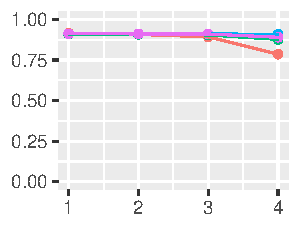
\includegraphics[height=2.4cm]{fig/vgg-fwd-skylake}
      & 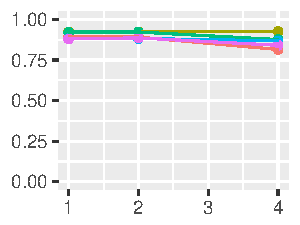
\includegraphics[trim=8mm 0mm 0mm 0mm,clip,height=2.4cm]{fig/vgg-upd-skylake}
      & 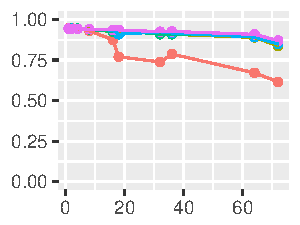
\includegraphics[trim=8mm 0mm 0mm 0mm,clip,height=2.4cm]{fig/vgg-fwd-haswell}
      & 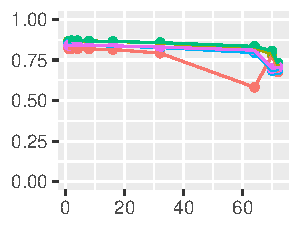
\includegraphics[trim=8mm 0mm 0mm 0mm,clip,height=2.4cm]{fig/vgg-upd-haswell}
      & 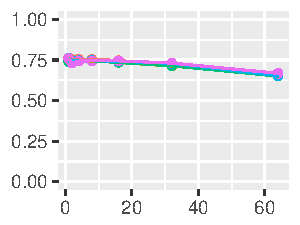
\includegraphics[trim=8mm 0mm 0mm 0mm,clip,height=2.4cm]{fig/vgg-fwd-knl}
      & 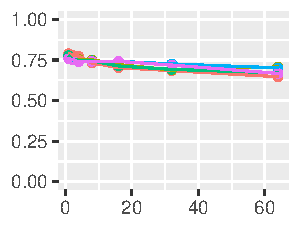
\includegraphics[trim=8mm 0mm 0mm 0mm,clip,height=2.4cm]{fig/vgg-upd-knl}
      & 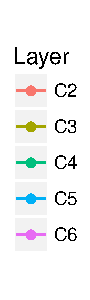
\includegraphics[height=2.4cm]{fig/vgg-legend} \\
      \midrule
      \rotatebox{90}{\qquad \textbf{U-Net}}
      & 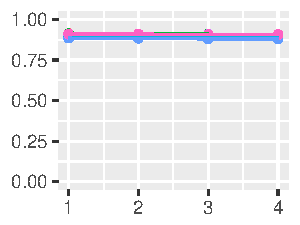
\includegraphics[height=2.4cm]{fig/unet-fwd-skylake}
      & 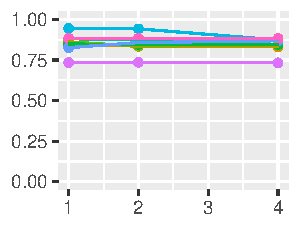
\includegraphics[trim=8mm 0mm 0mm 0mm,clip,height=2.4cm]{fig/unet-upd-skylake}
      & 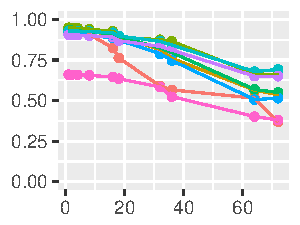
\includegraphics[trim=8mm 0mm 0mm 0mm,clip,height=2.4cm]{fig/unet-fwd-haswell}
      & 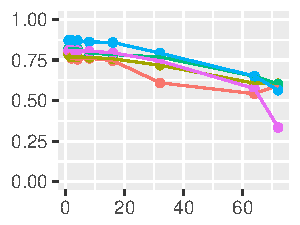
\includegraphics[trim=8mm 0mm 0mm 0mm,clip,height=2.4cm]{fig/unet-upd-haswell}
      & 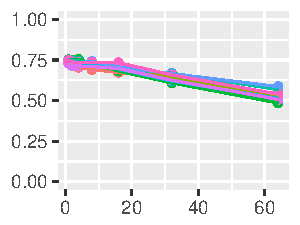
\includegraphics[trim=8mm 0mm 0mm 0mm,clip,height=2.4cm]{fig/unet-fwd-knl}
      & 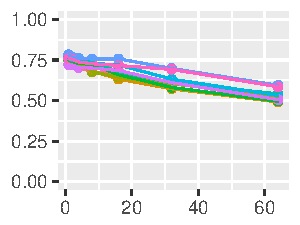
\includegraphics[trim=8mm 0mm 0mm 0mm,clip,height=2.4cm]{fig/unet-upd-knl}
      & 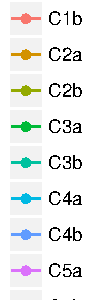
\includegraphics[height=2.4cm]{fig/unet-legend} \\
      \midrule
      \rotatebox{90}{\qquad \textbf{C3D}}
      & 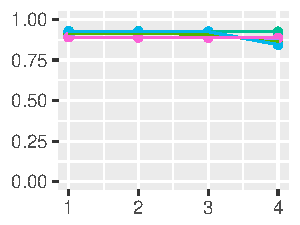
\includegraphics[height=2.4cm]{fig/d3d-fwd-skylake}
      & 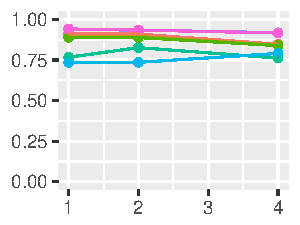
\includegraphics[trim=8mm 0mm 0mm 0mm,clip,height=2.4cm]{fig/d3d-upd-skylake}
      & 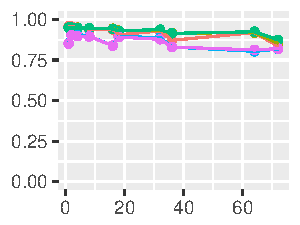
\includegraphics[trim=8mm 0mm 0mm 0mm,clip,height=2.4cm]{fig/d3d-fwd-haswell}
      & 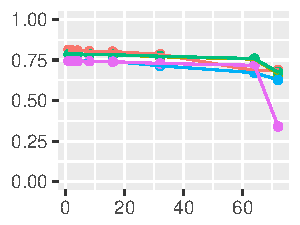
\includegraphics[trim=8mm 0mm 0mm 0mm,clip,height=2.4cm]{fig/d3d-upd-haswell}
      & 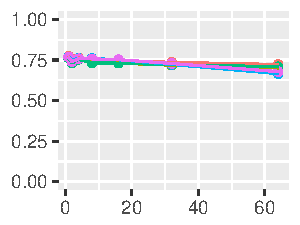
\includegraphics[trim=8mm 0mm 0mm 0mm,clip,height=2.4cm]{fig/d3d-fwd-knl}
      & 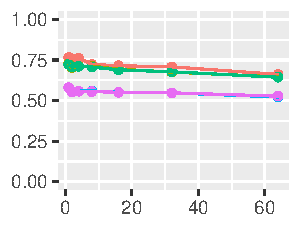
\includegraphics[trim=8mm 0mm 0mm 0mm,clip,height=2.4cm]{fig/d3d-upd-knl}
      & 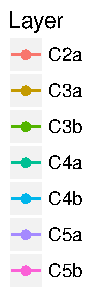
\includegraphics[height=2.4cm]{fig/d3d-legend} \\
      \midrule
      \rotatebox{90}{\qquad \textbf{Toy}}
      & 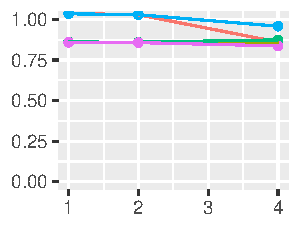
\includegraphics[height=2.4cm]{fig/toy-fwd-skylake}
      & 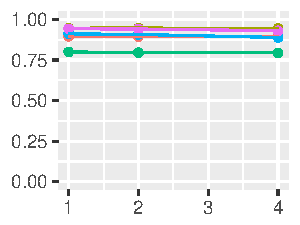
\includegraphics[trim=8mm 0mm 0mm 0mm,clip,height=2.4cm]{fig/toy-upd-skylake}
      & 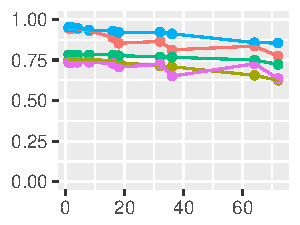
\includegraphics[trim=8mm 0mm 0mm 0mm,clip,height=2.4cm]{fig/toy-fwd-haswell}
      & 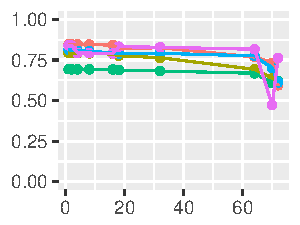
\includegraphics[trim=8mm 0mm 0mm 0mm,clip,height=2.4cm]{fig/toy-upd-haswell}
      & 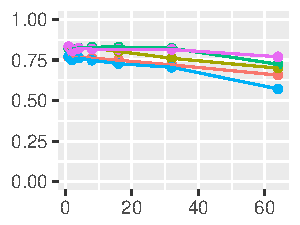
\includegraphics[trim=8mm 0mm 0mm 0mm,clip,height=2.4cm]{fig/toy-fwd-knl}
      & 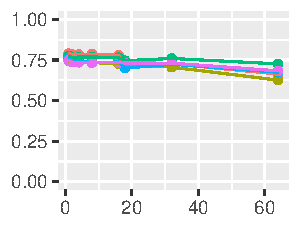
\includegraphics[trim=8mm 0mm 0mm 0mm,clip,height=2.4cm]{fig/toy-upd-knl}
      & 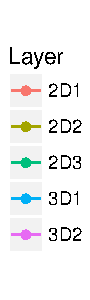
\includegraphics[height=2.4cm]{fig/toy-legend} \\
      \bottomrule

    \end{tabular}
    \caption{Scalability}
  \end{figure*}

  First, we demonstrate the near--linear scalability of our approach,
  regardless of the layer shape.  We show that our approach has the
  same utilization for all of them.

  Secondly, we compare the speed of our approach to alternative 2D
  primitives -- specifically CcT, MKL--DNN and MKL--2017.  We show
  that our approach is competitive, over--performing the next bet
  competitor by a small margin on Xeon and under--performing by a
  small margin on the KNL for 2D object--detection.  However, for
  semantical segmentation, we greatly outperform all competitors on
  both Xeon and Xeon Phi.

  Finally, we compare the speed of 3D networks to state of the art 3D
  primitives for the GPU.


  \begin{table} \centering
    \setlength\tabcolsep{2.5pt}
    \begin{tabular}{cr !{\vrule width0.8pt} rr|rr !{\vrule width0.8pt} rr|rr  }
      & & \multicolumn{4}{c !{\vrule width0.8pt} }{\textbf{cuDNNv5 (Titan X)}} & \multicolumn{4}{c}{\textbf{ZNNphi (Xeon)}} \\
      & & \multicolumn{2}{c|}{Maxwell} & \multicolumn{2}{c!{\vrule width0.8pt}}{Pascal}
      & \multicolumn{2}{c|}{Haswell} & \multicolumn{2}{c}{KNL} \\
      &  & Fwd & Bwd & Fwd & Bwd& Fwd & Bwd& Fwd & Bwd \\
      \hline
      \multirow{5}{*}{\rotatebox{90}{\textbf{C3D}}}
      & C2a & 186.8 & 370.3 & 168.0 & 336.0 & {\bf 147.6} & {\bf 325.2} & 218.1 & 456.3  \\
      & C3a & 90.1  & 180.0 & 78.5  & {\bf 161.2} & {\bf 72.2}  & 162.9 & 112.3 & 234.3  \\
      & C3b & 178.0 & 359.5 & 153.0 & 310.0 & {\bf 141.0} & {\bf 308.1} & 222.4 & 467.1  \\
      & C4a & 32.8  & 68.7  & 28.3  & {\bf 59.6}  & {\bf 27.7}  & 63.1  & 43.4  &  98.8  \\
      & C4b & 65.1  & 135.1 & 55.7  & {\bf 117.4} & {\bf 55.2}  & 131.2 & 85.3  & 196.1  \\
      \hline
    \end{tabular}
    \caption{3D vs GPU}
  \end{table}

  \begin{table} \centering
    \setlength\tabcolsep{2.5pt}
    \begin{tabular}{cr !{\vrule width0.8pt} rr|rr|rr|rr  }
      & & \multicolumn{2}{c|}{MKL-DNN} & \multicolumn{2}{c|}{MKL-2017}
      & \multicolumn{2}{c|}{CcT} & \multicolumn{2}{c}{ZNNPhi} \\
      &  & Fwd & Bwd & Fwd & Bwd& Fwd & Bwd& Fwd & Bwd \\
      \hline
      \multirow{5}{*}{\rotatebox{90}{\textbf{VGG-A}}}
      & C2  & 79.1  & 196.4 & 43.8 & 99.3  & 141.2 & 317.8 & {\bf 33.4} & {\bf 60.4}  \\
      & C3  & 42.4  & 106.8 & 30.0 & 78.5  & 118.5 & 194.3 & {\bf 24.5} & {\bf 60.3}  \\
      & C4  & 101.3 & 322.3 & 58.6 & 158.0 & 263.5 & 395.4 & {\bf 48.2} & {\bf 100.6} \\
      & C5  & 44.2  & 203.5 & 27.3 & 76.2  & 92.6  & 233.9 & {\bf 24.2} & {\bf 53.2}  \\
      & C6  & 89.8  & 466.5 & 54.8 & 149.9 & 196.8 & 466.3 & {\bf 47.2} & {\bf 104.2} \\
      \hline
      \multirow{5}{*}{\rotatebox{90}{\textbf{U-Net}}}
      & C1b  & 257.44 & 494.93 & 183.16 & 195.86 & 1739 &  542 & {\bf 9.02} & {\bf 18.12} \\
%%      & C2a  & 66.07  & 129.50 & 43.92  & 38.38  & 641  & 1199 & {\bf 3.80} & {\bf  8.51} \\
      & C2b  & 127.55 & 248.83 & 82.80  & 42.53  & 1052 & 1671 & {\bf 6.07} & {\bf 13.91} \\
%%      & C3a  & 36.47  & 67.78  & 21.64  & 13.08  & 1032 & 1627 & {\bf 3.55} & {\bf  8.88} \\
      & C3b  & 66.17  & 126.35 & 38.48  & 25.20  & 2988 & 4645 & {\bf 5.47} & {\bf 13.41} \\
%%      & C4a  & 21.04  & 40.69  & 11.50  & 13.80  & 693  & 1244 & {\bf 3.46} & {\bf  8.62} \\
      & C4b  & 53.89  & 90.54  & 18.66  & 26.90  & 2172 & 4033 & {\bf 5.16} & {\bf 13.21} \\
%%      & C5a  & 11.49  & 36.59  & 5.38   & 9.98   & 899  & 1754 & {\bf 3.23} & {\bf  8.12} \\
      & C5b  & 19.34  & 77.86  & 9.24   & 22.09  & 1667 & 3198 & {\bf 4.35} & {\bf 11.23} \\
      \hline

    \end{tabular}
    \caption{Haswell}
  \end{table}


  \begin{table} \centering
    \setlength\tabcolsep{2.5pt}
    \begin{tabular}{cr !{\vrule width0.8pt} rr|rr|rr  }
      & & \multicolumn{2}{c|}{MKL-DNN} & \multicolumn{2}{c|}{MKL-2017}
      & \multicolumn{2}{c}{ZNNPhi} \\
      &  & Fwd & Bwd& Fwd & Bwd& Fwd & Bwd \\
      \hline
      \multirow{5}{*}{\rotatebox{90}{\textbf{VGG-A}}}
      & C2  & 101.9 & 266.8 & {\bf 34.6} & 101.8 & 40.1 & {\bf  80.7}  \\
      & C3  & 72.5  & 192.3 & {\bf 32.9} & 87.1  & 39.7 & {\bf  76.8}  \\
      & C4  & 142.0 & 402.9 & {\bf 65.4} & 166.2 & 80.6 & {\bf 158.9}  \\
      & C5  & 53.0  & 268.5 & {\bf 32.8} & {\bf 72.9}  & 40.1 & 77.5   \\
      & C6  & 108.3 & 557.3 & {\bf 64.8} & {\bf 172.3} & 78.6 & 157.3  \\
      \hline
      \multirow{5}{*}{\rotatebox{90}{\textbf{U-Net}}}
      & C1b  & 799.60 & 1603.93 & 141.01 & 61.96 & {\bf 9.89} & {\bf 21.81} \\
%%      & C2a  & 195.82 & 410.73  & 41.90  & 19.20 & {\bf 5.27} & {\bf 11.19} \\
      & C2b  & 382.60 & 790.76  & 48.93  & 23.27 & {\bf 9.79} & {\bf 20.31} \\
%%      & C3a  & 96.19  & 212.08  & 11.97  & 10.01 & {\bf 5.13} & {\bf  9.77} \\
      & C3b  & 187.08 & 421.61  & 23.10  & 16.84 & {\bf 8.50} & {\bf 16.71} \\
%%      & C4a  & 48.05  & 110.39  & 5.60   & 23.26 & {\bf 4.44} & {\bf  9.32} \\
      & C4b  & 94.81  & 259.73  & 10.56  & 24.70 & {\bf 7.31} & {\bf 15.49} \\
%%      & C5a  & 25.17  & 90.04   & {\bf 3.66}   & 8.70  & 3.81 & {\bf  8.34} \\
      & C5b  & 44.01  & 167.88  & {\bf 5.45}   & {\bf 10.84} & 6.01 & 12.33 \\
      \hline

    \end{tabular}
    \caption{KNL}
  \end{table}
